% !TeX encoding = UTF-8
% !TeX spellcheck = de_DE
% !TeX program = lualatex
% !TeX BIB program = biber
%other magic comments: see TeXstudio user manual, chapter 4.10
\documentclass{standalone}

\usepackage{tikz}
\usetikzlibrary{circuits.ee.IEC}
\usepackage[compatibility]{circuitikz}

\title{Dreiwegeweiche}
\author{Wolfgang~Witt}
\date{\today}

\begin{document}
	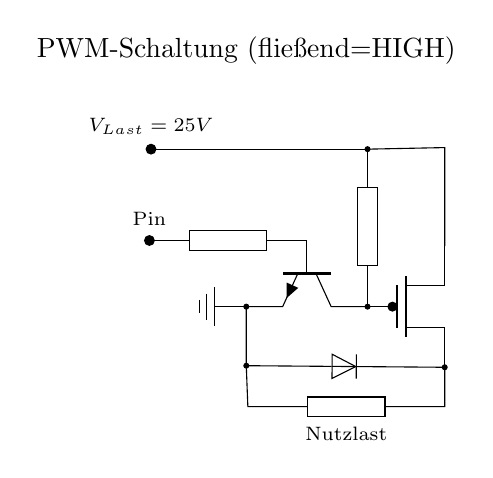
\begin{tikzpicture}[circuit ee IEC, every info/.style={font=\scriptsize}]
		\node (ground) [ground, rotate=180] {};
		\draw (ground) to ++(.5, 0) node (npn) [npn, anchor=emitter, rotate=-90] {};
		\node (contactE) at (npn.emitter) [contact, scale=.5] {};
		\draw (npn.base) to [resistor] ++(-2, 0) node (pin) [contact, info={Pin}] {};
		\node (contactC) at (npn.collector) [contact, scale=.5] {};
		\draw (contactC) to [resistor] ++(0, 2) node (contactV) [contact, scale=.5] {} to ++(-2.75,0) node (Vcc) [contact, info={$V_{Last}=25V$}] {};
		\node (fet) [pmos, anchor=gate] at (contactC) {};
		\draw (fet.source) to ++(0, 1.25) to (contactV);
		\node (contactF) [contact, scale=.5] at (fet.drain) {};
		\draw (contactE) to ++(0, -.75) node (contactG) [contact, scale=.5] {} to [diode] (contactF);
		\draw (contactF) to ++(0, -.5) to [resistor={info={Nutzlast}}] ++(-2.5, 0) to (contactG);
		%Überschrift
		\path (ground) ++(.5, 3.25) node {PWM-Schaltung (fließend=HIGH)};
	\end{tikzpicture}
\end{document}
